% Le verre taillé — document de recherche.
%
% Tout chiffre de ce document provient d'un essai lancé sur la machine
% décrite au §2. Les sources des bancs sont dans recherche/verre-taille.
% Compilation : latexmk -pdf verre-taille.tex

\documentclass[11pt,a4paper]{article}

\usepackage[T1]{fontenc}
\usepackage[utf8]{inputenc}
\usepackage[french]{babel}
\usepackage{lmodern}
\usepackage{microtype}
\usepackage[a4paper,margin=3cm]{geometry}
\usepackage{booktabs}
\usepackage{graphicx}
\usepackage{tikz}
\usepackage{pgfplots}
\usepackage{amsmath}
\usepackage{caption}
\usepackage[hidelinks]{hyperref}

\pgfplotsset{compat=1.18}
\usetikzlibrary{positioning,arrows.meta,calc}

\captionsetup{font=small,labelfont=bf}
\setlength{\parskip}{0.4em}
\setlength{\parindent}{0pt}

\newcommand{\uni}[1]{\texttt{#1}}
% Les nombres sont déjà écrits à la française dans le source ; cette commande
% ne sert qu'à les marquer comme mesures, pour pouvoir les traiter un jour.
\newcommand{\np}[1]{#1}

\title{\textbf{Le verre taillé}\\[0.3em]
\large Une matière translucide de forme libre sous Windows,\\
obtenue en cessant de la demander au compositeur}
\author{Ariel Stone}
\date{12 septembre 2026}

\begin{document}
\maketitle

\begin{abstract}
\noindent
Windows~11 sait poser un fond translucide derrière une fenêtre, mais ce fond
est un rectangle que rien ne découpe~: ni la transparence par pixel, ni la
région de fenêtre. Une interface dont l'élément flottant n'est pas
rectangulaire ne peut donc pas s'en servir. Ce document décrit une autre voie,
mesurée de bout en bout~: la fenêtre se déclare invisible à la capture d'écran,
capture ce qui se trouve derrière elle, le floute elle-même sur le processeur
graphique, et le masque par sa propre forme. La question qui décide — une
fenêtre qui se capture se voit-elle elle-même~? — est tranchée par un essai à
témoin~: \textbf{115\,200} pixels témoins sans le drapeau d'exclusion,
\textbf{0} avec. Sur les mêmes fonds de référence, et à lisibilité égale avec
le fond du système (contraste de \np{12,00} contre \np{12,2}), la matière
obtenue laisse passer \textbf{trois fois et demie} plus de l'arrière-plan. Elle
atteint le noir véritable là où le fond du système plafonne à un gris, et elle
ne dépend d'aucun réglage que le système peut couper. Son coût est de
\np{0,9}~ms par trame au repos.
\end{abstract}

\tableofcontents
\bigskip
\hrule

\section{Le problème}

Une veilleuse d'étude affiche, par-dessus les autres fenêtres, un îlot
flottant qui porte le temps restant. Cet îlot a une forme~: un galet à coins
très arrondis, dont la spécification interdit qu'il dessine un cadre
rectangulaire dans une chambre sombre.

La demande était que cet îlot soit en verre. Le chemin évident consiste à
demander à Windows son fond translucide, par l'attribut documenté
\uni{DWMWA\_SYSTEMBACKDROP\_TYPE} ou par la politique d'accentuation non
documentée. Les deux fonctionnent. Aucun des deux ne convient, et la raison
n'est pas celle qu'on attend.

\section{La machine, et la méthode}

\subsection{La machine}

\begin{center}
\begin{tabular}{ll}
\toprule
système & Windows~11 Pro, 10.0.26200 \\
processeurs graphiques & Intel UHD intégré et NVIDIA RTX~4060 portable \\
chaîne & Rust 1.98.1, \uni{stable-x86\_64-pc-windows-msvc} \\
rendu & \uni{wgpu}~30.0.1 sur Vulkan \\
\bottomrule
\end{tabular}
\end{center}

\subsection{La méthode}

Trois règles gouvernent tout ce document, et elles ont été payées~:

\begin{enumerate}
\item \textbf{Une affirmation sans mesure n'existe pas.} Chaque chiffre
provient d'un programme lancé sur cette machine, avec l'image qui le prouve.
\item \textbf{Une mesure doit avoir son témoin}, c'est-à-dire un cas dont la
réponse est connue d'avance. Sans témoin, un résultat nul se confond avec un
instrument qui ne mesure rien. Le §\ref{sec:exclusion} en donne l'exemple le
plus net.
\item \textbf{Ce qui n'a pas été mesuré s'écrit comme non mesuré.} Le
§\ref{sec:limites} rassemble les trous, nommés.
\end{enumerate}

\section{Ce que le fond du système donne, et ses cinq limites}

Les deux voies ont été éprouvées, sur six combinaisons de dorsal et
d'adaptateur, avec 126~images de contrôle. Le fond translucide existe bien sur
cette machine. Cinq mesures montrent qu'il ne convient pas à cet îlot.

\subsection{Il est rectangulaire, et rien ne le découpe}
\label{sec:rectangle}

C'est le résultat qui décide, et il n'était pas prévu. Le compositeur de
bureau traite le fond de système comme un \emph{visuel séparé}, placé
\emph{sous} la surface de l'application. Trois conséquences, toutes vérifiées~:

\begin{itemize}
\item la transparence par pixel ne le soustrait pas. Elle dit quelle part de
\emph{notre} encre couvre le fond, jamais l'inverse~: un galet noir peint sur
le verre laisse les quatre coins du rectangle \emph{remplis de verre}~;
\item la découpe de fenêtre ne l'entame pas davantage. Elle ne s'applique qu'à
notre surface, et le verre reste carré~;
\item posée \emph{après} l'effet, la découpe le détruit~: dalle noire opaque
sur une voie, gris uni sur l'autre.
\end{itemize}

Il n'existe pas de découpe par pixel sous Windows. Donc~: \textbf{verre
rectangulaire à coins carrés, ou pas de verre du système.}

\subsection{Les quatre autres}

\begin{center}
\begin{tabular}{ll}
\toprule
plancher de noir & \uni{\#212224}, jamais le noir véritable \\
contraste d'un blanc chaud posé dessus & tombe de \np{18,30} à \np{1,29} \\
grain & présent, aucun réglage ne l'enlève \\
coupure automatique & à 20\,\% de batterie \\
\bottomrule
\end{tabular}
\end{center}

La coupure mérite d'être détaillée, parce qu'elle survient précisément quand
on en a le moins besoin, c'est-à-dire en fin de nuit sur un portable. Et sa
détection réserve un piège traité au §\ref{sec:disponibilite}.

\section{La voie inverse~: tailler son propre verre}

Puisque le fond du système est un rectangle indécoupable, on ne le demande
plus. On le fabrique.

\begin{center}
\begin{tikzpicture}[
  node distance=6mm,
  etape/.style={draw,rounded corners=2pt,align=center,inner sep=5pt,
                font=\small,minimum height=11mm,text width=27mm},
  fleche/.style={-{Stealth[length=2mm]},thick}
]
\node[etape] (a) {fenêtre invisible\\à la capture};
\node[etape,right=of a] (b) {capture de la\\région derrière};
\node[etape,right=of b] (c) {flou séparable\\en linéaire};
\node[etape,below=8mm of c] (d) {teinte sur les\\octets encodés};
\node[etape,left=of d] (e) {masque\\superellipse};
\node[etape,left=of e] (f) {l'îlot};
\draw[fleche] (a) -- (b);
\draw[fleche] (b) -- (c);
\draw[fleche] (c) -- (d);
\draw[fleche] (d) -- (e);
\draw[fleche] (e) -- (f);
\end{tikzpicture}
\captionof{figure}{La chaîne. Le compositeur du système n'intervient nulle
part. Les deux maillons soulignés au §\ref{sec:espaces} sont ceux qui décident
de la lisibilité.}
\end{center}

\section{La preuve qui conditionne tout le reste}
\label{sec:exclusion}

L'objection immédiate est fatale si elle tient~: une fenêtre qui capture ce qui
est derrière elle se capture elle-même, et l'image boucle sur son propre reflet
jusqu'à saturer.

Windows offre la sortie depuis la version~2004~: une fenêtre peut se déclarer
invisible à la capture d'écran tout en restant visible à l'\oe il. Reste à
savoir si cela vaut pour la duplication de bureau, qui est le chemin rapide.

\subsection{Le protocole, et pourquoi il a un témoin}

Une fenêtre d'une couleur que rien d'autre ne porte à l'écran, de
$480 \times 240$ pixels, posée en $(400, 300)$. Le bureau est capturé
\emph{deux fois}~: sans le drapeau d'exclusion, puis avec. On compte les pixels
de la couleur témoin.

\begin{center}
\begin{tabular}{lrl}
\toprule
& pixels témoins & premier pixel \\
\midrule
sans exclusion & \textbf{115\,200} & $(400, 300)$ \\
avec exclusion & \textbf{0} & --- \\
\bottomrule
\end{tabular}
\end{center}

\np{115200} est exactement $480 \times 240$, et le premier pixel tombe
exactement où la fenêtre est posée. \textbf{Le premier essai prouve que
l'instrument voit ce qu'il doit voir}~; le second prouve que l'exclusion est
totale.

Sans le témoin, le zéro de la seconde ligne n'aurait rien voulu dire~: il se
confond avec un test qui ne mesure rien. C'est la leçon la plus transposable
de ce travail.

\section{Trois pièges de la duplication de bureau}

Aucun des trois ne se voit à la lecture du code, et chacun coûte une séance
entière.

\subsection{La conscience de la résolution}

Sans elle, déclarée \emph{avant} toute fenêtre et toute initialisation
graphique, les coordonnées du bureau reviennent mises à l'échelle
($1536 \times 864$) alors que la texture est en pixels physiques
($1920 \times 1080$). Les deux nombres ont l'air corrects séparément, et tout
tombe à côté.

\subsection{L'horodatage de présentation}

L'acquisition d'une trame réussit aussi quand \emph{seul le curseur a bougé},
et la texture rendue ne contient alors aucune image neuve. Le seul signal
fiable est l'horodatage de dernière présentation. Sans ce contrôle, on lit du
hasard.

\subsection{La libération de la trame}
\label{sec:release}

Libérer la trame rend le contenu de sa texture \emph{indéfini}. La copie doit
avoir lieu \textbf{avant}. En la faisant après, on lit un noir parfait, de
moyenne exactement $(0{,}0\,;\,0{,}0\,;\,0{,}0)$, et l'on conclut que la
duplication ne fonctionne pas sur cette machine. C'est la faute qui a coûté le
plus cher ici, parce que son symptôme ressemble à une panne matérielle.

\medskip
Enfin, la duplication ne rend que les \emph{changements}. Un bureau immobile
n'en produit aucun et l'appel expire, ce qui ressemble encore à une panne. Tout
banc de mesure a donc besoin d'un agitateur~: quelque chose qui bouge pour
forcer une présentation.

\section{Les deux espaces colorimétriques}
\label{sec:espaces}

C'est la découverte de ce travail, et elle était contre-intuitive.

Le flou est une \textbf{moyenne physique}~: il doit se faire là où la lumière
s'additionne, c'est-à-dire en espace linéaire. Les textures étant vues en
sRGB, l'échantillonnage décode et l'écriture réencode, et la somme gaussienne
a lieu au bon endroit sans effort. Le compositeur du système, lui, mélange sur
les octets stockés.

La teinte, elle, ne doit \textbf{pas} suivre le flou. C'est un geste de
peintre, qui se juge là où l'\oe il juge, donc sur les octets encodés. À
teinte égale, le même mélange donne~:

\begin{center}
\begin{tabular}{lr}
\toprule
teinte noire à \np{0,80}, sur un fond de valeur 226 & résultat \\
\midrule
mélangée en linéaire & 109 \\
mélangée sur les octets encodés & \textbf{45} \\
\bottomrule
\end{tabular}
\end{center}

Séparer les deux espaces n'est pas un détail de réglage~: c'est ce qui décide
si la matière est lisible ou délavée.

\section{Mesures}

\subsection{Le critère, et pourquoi le flou ne suffit pas}

Montrer qu'un motif fin disparaît ne prouve rien. Un motif qui disparaît est
une preuve d'\emph{opacité}, pas de verre. Une vraie matière translucide fait
deux choses \emph{ensemble}~: elle efface le motif fin \textbf{et} elle porte
la luminance d'ensemble de ce qui est derrière.

On mesure donc toujours les deux~:
\begin{itemize}
\item l'\textbf{énergie de haute fréquence}, moyenne des sauts entre pixels
voisins, qui dit si le flou a eu lieu~;
\item la \textbf{porte}, écart de luminance de la matière entre un fond clair
et un fond sombre, qui dit ce qui traverse.
\end{itemize}

\subsection{La table de décision}

Fonds unis de valeurs 226 et 37, soit un écart de luminance de 189, choisis
pour être identiques à ceux des mesures du fond de système. Les trois dernières
colonnes donnent le contraste des trois encres de la charte.

\begin{center}
\small
\begin{tabular}{llrrrrrr}
\toprule
teinte & espace & clair & sombre & porte & \uni{\#F2EFE9} & \uni{\#8E8B86} & \uni{\#5E5B57} \\
\midrule
\np{0,70} & linéaire & 132 & 17 & \np{115,0} & \np{3,26} & \np{1,10} & \np{1,81} \\
\np{0,80} & linéaire & 109 & 12 & \np{97,0} & \np{4,51} & \np{1,52} & \np{1,30} \\
\np{0,86} & linéaire & 92 & 9 & \np{83,0} & \np{5,83} & \np{1,97} & \np{1,01} \\
\np{0,90} & linéaire & 78 & 6 & \np{72,0} & \np{7,25} & \np{2,45} & \np{1,23} \\
\np{0,96} & linéaire & 49 & 3 & \np{46,0} & \np{11,34} & \np{3,83} & \np{1,93} \\
\midrule
\np{0,70} & octets & 68 & 11 & \np{57,0} & \np{8,49} & \np{2,87} & \np{1,44} \\
\textbf{\np{0,80}} & \textbf{octets} & \textbf{45} & \textbf{7} & \textbf{\np{38,0}} & \textbf{\np{12,00}} & \textbf{\np{4,06}} & \textbf{\np{2,04}} \\
\np{0,86} & octets & 32 & 5 & \np{27,0} & \np{14,20} & \np{4,80} & \np{2,41} \\
\np{0,90} & octets & 23 & 4 & \np{19,0} & \np{15,62} & \np{5,28} & \np{2,66} \\
\np{0,93} & octets & 16 & 3 & \np{13,0} & \np{16,58} & \np{5,61} & \np{2,82} \\
\midrule
\np{1,00} & --- & 0 & 0 & \np{0,0} & \np{18,30} & \np{6,19} & \np{3,11} \\
\bottomrule
\end{tabular}
\end{center}

\subsection{La comparaison qui compte}

Le fond de système, réglé à la seule teinte que la charte supporte, donne un
contraste de \np{12,2} sur le blanc chaud pour une porte de \np{10,8}. La
ligne en gras ci-dessus donne \np{12,00} de contraste pour une porte de
\np{38,0}.

\begin{center}
\begin{tikzpicture}
\begin{axis}[
  width=12cm, height=7.5cm,
  xlabel={contraste de l'encre claire \uni{\#F2EFE9}},
  ylabel={porte (niveaux de luminance)},
  xmin=2, xmax=19, ymin=-5, ymax=125,
  grid=major, grid style={gray!25},
  legend pos=north east, legend cell align=left,
  every axis plot/.append style={thick},
  label style={font=\small}, tick label style={font=\small},
  legend style={font=\small}
]
\addplot[mark=*,mark size=1.6pt,color=black!55] coordinates {
  (3.26,115.0) (4.51,97.0) (5.83,83.0) (7.25,72.0) (8.89,61.0) (11.34,46.0) (18.30,0)
};
\addlegendentry{teinte en linéaire}
\addplot[mark=square*,mark size=1.6pt,color=black] coordinates {
  (8.49,57.0) (12.00,38.0) (14.20,27.0) (15.62,19.0) (16.58,13.0) (17.35,7.0) (18.30,0)
};
\addlegendentry{teinte sur les octets}
\addplot[only marks,mark=triangle*,mark size=3.5pt,color=black] coordinates {(12.2,10.8)};
\addlegendentry{fond du système}
\draw[dashed,gray] (axis cs:12.0,-5) -- (axis cs:12.0,38.0);
\draw[dashed,gray] (axis cs:2,38.0) -- (axis cs:12.0,38.0);
\draw[dashed,gray] (axis cs:2,10.8) -- (axis cs:12.2,10.8);
\end{axis}
\end{tikzpicture}
\captionof{figure}{À contraste égal, ce qui traverse la matière. La verticale
en tirets marque le contraste du fond de système~; à cette abscisse, la
matière taillée porte \np{38,0} niveaux contre \np{10,8}.}
\end{center}

Le flou est réel par ailleurs~: l'énergie de haute fréquence tombe de
\np{47,32} derrière la matière à \np{1,02} dedans, soit un facteur~46.

\subsection{Ce que les images montrent}

\begin{center}
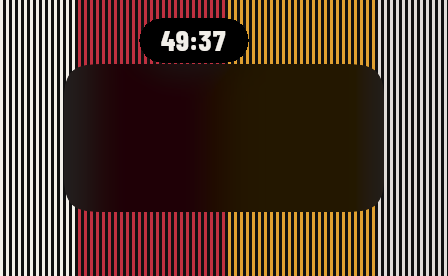
\includegraphics[width=0.48\textwidth]{../recherche/verre-taille/captures/verre-octets-80.png}
\hfill

\includegraphics[width=0.48\textwidth]{../recherche/verre-taille/captures/opaque.png}
\captionof{figure}{À gauche la matière taillée, teinte \np{0,80} sur les
octets~; à droite le galet opaque. Même planche rayée. Les rayures
disparaissent dedans et restent nettes dehors, et la matière porte la couleur
de la bande qu'elle recouvre.}
\end{center}

\section{Le régime continu}

Le coût d'une image ne dit rien du coût d'une seconde. L'acquisition doit être
\textbf{non bloquante}~: attendre une trame du bureau dans la boucle de rendu
reviendrait à caler l'affichage sur l'activité des autres fenêtres.

\subsection{Le filtre sans lequel tout est gaspillé}

Le premier banc rapportait 99\,\% de trames recopiées alors que le bureau était
censé être immobile. Le résultat n'avait pas de sens, et c'est lui qui a mis
sur la piste~: l'acquisition se réveille pour \emph{tout l'écran}, pas pour la
région suivie. Une horloge changeant de minute dans un coin faisait recopier
483~kilo-octets.

Le système dit pourtant quelles zones ont bougé, par les rectangles
\emph{sales} et les rectangles de \emph{déplacement}. En ne recopiant que si
l'un d'eux croise la région~:

\begin{center}
\begin{tabular}{lrr}
\toprule
bureau calme & avant & après \\
\midrule
trames recopiées & 99\,\% & \textbf{1\,\%} \\
coût d'un tour à vide & \np{0,380}~ms & \textbf{\np{0,060}~ms} \\
\bottomrule
\end{tabular}
\end{center}

Le cas animé continue de détecter 99\,\%, donc le filtre ne laisse pas passer
de matière périmée.

\textbf{La règle de prudence n'est pas symétrique}, et doit être écrite dans le
code~: en cas de doute, la réponse est \emph{oui, la région est touchée}. Un
faux positif coûte une copie~; un faux négatif laisse à l'écran une matière qui
ment.

\subsection{Le coût}

\begin{center}
\begin{tabular}{lrrr}
\toprule
& bureau calme & bureau animé & îlot en déplacement \\
\midrule
trames avec image neuve & 1 à 16\,\% & 100\,\% & 99\,\% \\
copie, médiane & \np{0,83}~ms & \np{1,17}~ms & \np{1,36}~ms \\
tour à vide, médiane & \np{0,060}~ms & --- & \np{0,096}~ms \\
accès perdus sur 9~s & 0 & 0 & 0 \\
\bottomrule
\end{tabular}
\end{center}

Le rendu lui-même — deux passes de flou et la composition — a d'abord été
annoncé à \np{0,82}~ms dans ce document. \textbf{Ce chiffre portait un nom
faux}~: il comptait aussi l'allocation de quatre textures, le téléversement de
la région et la relecture vers le processeur, dont l'application ne fait rien
par trame. Remesuré en séparant les deux, le rendu seul vaut \np{0,215}~ms et
l'aller-retour complet \np{0,465}~ms.

Ni l'un ni l'autre ne reproduit \np{0,82}~ms, et \textbf{l'écart n'est pas
expliqué}. Il est dit tel quel plutôt que de retenir celui qui arrange. Ce qui
est acquis, c'est que le coût réel de l'effet est \emph{inférieur} à ce qui
avait été publié.

Le total par trame va de \textbf{\np{0,9}~ms} au repos à \textbf{\np{2,2}~ms}
dans le pire cas, pour un budget de \np{6,94}~ms à 144~Hz.

Le premier chiffre varie d'un lancement à l'autre, entre 1 et 16\,\%, et c'est
normal~: il dépend de ce qui vit sur le bureau à cet instant. Un bureau
véritablement immobile n'existe pas sur une machine en service.

\subsection{Le déplacement demande sa propre règle}

Quand l'îlot bouge, la région suivie change, et aucun rectangle sale ne peut
dire ce qui se trouve sous la \emph{nouvelle} position. Il faut alors forcer
une copie sans attendre de trame neuve. S'il n'y en a pas, on garde la
précédente~: mieux vaut un retard d'une trame qu'un à-coup dans le
déplacement.

\section{Un signal qui ressemble au bon et n'en est pas}
\label{sec:disponibilite}

La coupure des effets de transparence par l'économiseur d'énergie ne touche
\emph{pas} le registre. Lire le réglage manuel ne suffit donc pas.

Une fonction du compositeur renvoie un drapeau d'opacité qui vaut vrai pendant
la coupure. Il ressemble au signal cherché. Il n'en est pas un~: il vaut
\emph{aussi} vrai machine sur secteur, économiseur éteint, effet parfaitement
vivant. Il décrit l'opacité de la couleur d'accentuation, pas la disponibilité
de la composition. Une fonction qui exigerait sa négation renverrait faux en
permanence.

\begin{quote}
Une observation faite pendant une panne n'est une cause que si on la vérifie
\emph{aussi} hors panne.
\end{quote}

La détection correcte demande deux signaux, dont aucun ne suffit seul~: l'état
de l'économiseur d'énergie, et le réglage manuel de transparence.

\section{La forme}

Le masque est une distance signée, donc un calcul par pixel~: rien à demander
au compositeur. La différence entre un coin en arc de cercle et un coin
continu tient dans une seule norme, celle d'ordre~$n$ au lieu de la norme
euclidienne.

Ce que le chiffre montre, et qu'aucun mot ne remplace~: à $n = 2$, la courbure
le long du quart de coin \textbf{saute} de 0 à $1/r$ à l'endroit exact où la
droite rencontre la courbe. Pour tout $n > 2$, elle part de zéro et monte
progressivement.

\begin{center}
\small
\begin{tabular}{lrrrrr}
\toprule
$n$ & $t = 0$ & $t = 0{,}05$ & $t = 0{,}20$ & $t = 0{,}50$ & $t = 1$ \\
\midrule
\np{2,0} & \np{0,0357} & \np{0,0357} & \np{0,0357} & \np{0,0357} & \np{0,0357} \\
\np{2,5} & \np{0,0000} & \np{0,0104} & \np{0,0210} & \np{0,0350} & \np{0,0500} \\
\np{3,0} & \np{0,0000} & \np{0,0028} & \np{0,0114} & \np{0,0303} & \np{0,0636} \\
\np{4,0} & \np{0,0000} & \np{0,0002} & \np{0,0030} & \np{0,0198} & \np{0,0901} \\
\bottomrule
\end{tabular}
\captionof{table}{Courbure le long du quart de coin, rayon 28~px. $t = 0$ est
la jonction avec le bord droit, où la courbure devrait être nulle.}
\end{center}

Deux pièges accompagnent ce changement~:

\begin{itemize}
\item la norme d'ordre~$n$ n'est pas une distance euclidienne. Son gradient
vaut $2^{1/n - 1/2}$ vers 45 degrés, soit \np{0,841} pour $n = 4$. Sans
division par ce gradient, le pixel de transition s'épaissit de 19\,\% à la
pointe du coin, et le bord y paraît flou alors qu'il est net ailleurs~;
\item la puissance n'est pas définie sur une valeur négative, d'où la coupure à
zéro \emph{avant} de l'appliquer.
\end{itemize}

\section{Limites, et ce qui n'a pas été mesuré}
\label{sec:limites}

Aucun des points suivants n'est un obstacle connu. Ce sont des trous, et les
nommer vaut mieux que de les laisser se découvrir en marche.

\begin{itemize}
\item \textbf{Les pannes de la duplication.} Elle perd son accès au changement
de mode d'affichage, sur le bureau sécurisé, et devant une application en
plein écran exclusif. Le code qui la rouvre existe~; aucune panne ne s'est
produite pendant les essais, donc ce chemin n'a jamais tourné pour de vrai.
\item \textbf{Le contenu protégé} rend du noir. Acceptable, mais à dire.
\item \textbf{La consommation} sur batterie n'a pas été chiffrée.
\item \textbf{Le réveil parasite.} Depuis une version récente de Windows~11,
l'acquisition se réveille aussi quand la fenêtre exclue se met à jour, même si
son contenu n'est pas capturé. Du travail pour rien, à éviter.
\item \textbf{Le repli sans transparence par pixel.} Sur un adaptateur dont la
surface ne l'annonce pas, on peut peindre hors de la forme les pixels capturés
eux-mêmes, ce qui donne une transparence parfaite tant que le fond ne bouge
pas. Non essayé.
\item \textbf{La matière du bord} — réfraction, réflectance, dispersion — fait
l'objet d'un travail séparé et n'est pas décrite ici.
\end{itemize}

\section{Conclusion}

La limite rencontrée n'était pas celle qu'on croyait. Le fond translucide du
système n'est pas insuffisant~: il est \emph{rectangulaire}, et cette propriété
seule interdit toute interface dont l'élément flottant a une forme. Aucun
réglage ne la contourne, parce qu'elle vient de l'architecture du compositeur.

En cessant de demander la matière et en la fabriquant, on récupère la forme,
le noir véritable, l'indépendance aux réglages du système, et un contrôle
complet du compromis entre translucidité et lisibilité — compromis qui ne
disparaît pas, car il est physique, mais qui cesse d'être subi.

Le prix est de \np{0,9}~ms par trame au repos, et une discipline~: recopier
seulement quand la région a réellement changé.

\bigskip
\hrule
\medskip
\small
\textbf{Reproductibilité.} Les bancs de mesure de ce document sont dans
\uni{recherche/verre-taille}~: \uni{sonde.rs} pour la preuve d'exclusion,
\uni{bureau.rs} pour la capture, \uni{verre.wgsl} et \uni{verre.rs} pour la
matière et ses mesures, \uni{regime.rs} pour le coût en marche. Chacun écrit
les images qui accompagnent ses chiffres.

\end{document}
